% 1977 年新疆卷（文科）第四题：四边形 ABCD，E、F、M、N 分别为 AD、AB、BC、CD 的中点，
% 实线 EM 与 FN，虚线 EF、FM、MN、NE 及对角线 BD（按源卷第 3 页布局：A 左上、D 右上、B 左下、C 右下）
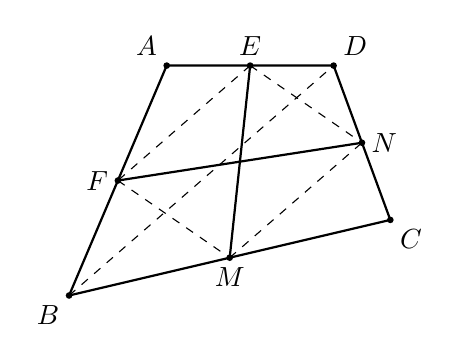
\begin{tikzpicture}[scale=1.0]
  \coordinate (B) at (0,0);
  \coordinate (A) at (1.24,2.92);
  \coordinate (D) at (3.36,2.92);
  \coordinate (C) at (4.08,0.96);
  \coordinate (E) at (2.30,2.92);
  \coordinate (F) at (0.62,1.46);
  \coordinate (M) at (2.04,0.48);
  \coordinate (N) at (3.72,1.94);
  \draw[thick] (A)--(D)--(C)--(B)--cycle;
  \draw[thick] (E)--(M);
  \draw[thick] (F)--(N);
  \draw[dashed] (E)--(F);
  \draw[dashed] (E)--(N);
  \draw[dashed] (F)--(M);
  \draw[dashed] (M)--(N);
  \draw[dashed] (B)--(D);
  \fill (A) circle (1.2pt) node[above left] {$A$};
  \fill (D) circle (1.2pt) node[above right] {$D$};
  \fill (C) circle (1.2pt) node[below right] {$C$};
  \fill (B) circle (1.2pt) node[below left] {$B$};
  \fill (E) circle (1.2pt) node[above] {$E$};
  \fill (F) circle (1.2pt) node[left] {$F$};
  \fill (M) circle (1.2pt) node[below] {$M$};
  \fill (N) circle (1.2pt) node[right] {$N$};
\end{tikzpicture}
